\documentclass[a4paper,12pt]{article}

\usepackage{geometry}
\geometry{margin=2.5cm}
\usepackage{graphicx}
\usepackage{xcolor}
\usepackage{fontspec}       % Nécessaire pour utiliser Marianne
\usepackage{setspace}
\usepackage{ragged2e}

% Déclaration de la police Marianne (si elle est bien installée sur ton système)
\newfontfamily\marianne{Marianne}

% Couleur bleue officielle (ajustable si besoin)
\definecolor{etatbleu}{RGB}{15,36,62}

\begin{document}

\begin{titlepage}
    \centering

    % Logos en haut
    \begin{minipage}{0.45\textwidth}
        \raggedright
        
\includegraphics[width=4cm]{./ressources/logo_cnig.png}
    \end{minipage}
    \hfill
    \begin{minipage}{0.45\textwidth}
        \raggedleft
        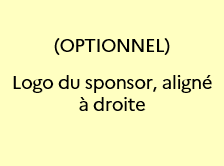
\includegraphics[width=4cm]{./ressources/logo_sponsor.PNG}
    \end{minipage}

    \vspace{1cm}

    % Titre haut centré
    {\marianne\large\color{etatbleu} Conseil national de l'information Géolocalisée\par}

    \vspace{1.5cm}

    % Image centrale
    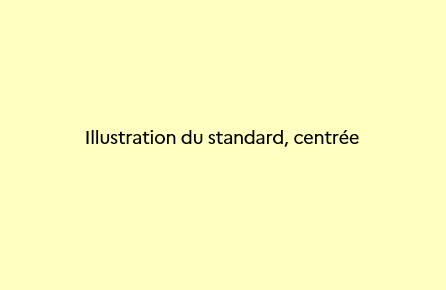
\includegraphics[width=5cm]{./ressources/illustration_standard.PNG}

    \vspace{1.5cm}

    % Titre principal en Marianne + bleu
    {\marianne\fontsize{27pt}{26pt}\selectfont\color{etatbleu} Géostandards Risques\par}

    \vspace{0.5cm}

    % Sous-titre en Marianne + bleu
    {\marianne\large\color{etatbleu} Plans de prévention des risques (PPR)\par}

    \vspace{1cm}

    % Abstract
    {\marianne\normalsize Abstract\par}

    \vspace{5cm}

    % Pied de page
    {\marianne\small\itshape Groupe de travail refonte des Géostandards Risques\par}
    \vspace{0.3cm}
    {\marianne\small\itshape Version 0.2 - Date\par}


\end{titlepage}

\newpage
\thispagestyle{empty}
\mbox{}
\newpage

\end{document}
